%%%%%%%%%%%%%%%%%%%%%%%%%%%%%%%%%%%%%%%%%
% Databases Report
%%%%%%%%%%%%%%%%%%%%%%%%%%%%%%%%%%%%%%%%%

%----------------------------------------------------------------------------------------
%	PACKAGES AND OTHER DOCUMENT CONFIGURATIONS
%----------------------------------------------------------------------------------------

\documentclass{article}

\usepackage{fancyhdr} % Required for custom headers
\usepackage{lastpage} % Required to determine the last page for the footer
\usepackage{extramarks} % Required for headers and footers
\usepackage[usenames,dvipsnames]{color} % Required for custom colors
\usepackage{graphicx} % Required to insert images
\usepackage{listings} % Required for insertion of code
\usepackage{courier} % Required for the courier font
\usepackage{url}
\usepackage{etoolbox}
\patchcmd{\thebibliography}{\section*{\refname}}{}{}{}

% Margins
\topmargin=-0.45in
\evensidemargin=0in
\oddsidemargin=0in
\textwidth=6.5in
\textheight=9.0in
\headsep=0.25in

\linespread{1.1} % Line spacing

% Set up the header and footer
\pagestyle{fancy}
%\lhead{\hmwkAuthorName} % Top left header
%\chead{\hmwkClass\  \hmwkTitle} % Top center head
%\rhead{\firstxmark} % Top right header
\lfoot{\lastxmark} % Bottom left footer
\cfoot{} % Bottom center footer
\rfoot{Page\ \thepage\ of\ \protect\pageref{LastPage}} % Bottom right footer
\renewcommand\headrulewidth{0.4pt} % Size of the header rule
\renewcommand\footrulewidth{0.4pt} % Size of the footer rule

\setlength\parindent{0pt} % Removes all indentation from paragraphs

%----------------------------------------------------------------------------------------
%	CODE INCLUSION CONFIGURATION
%----------------------------------------------------------------------------------------

\definecolor{MyDarkGreen}{rgb}{0.0,0.4,0.0} % This is the color used for comments
\lstloadlanguages{Perl} % Load Perl syntax for listings, for a list of other languages supported see: ftp://ftp.tex.ac.uk/tex-archive/macros/latex/contrib/listings/listings.pdf
\lstset{language=Perl, % Use Perl in this example
        frame=single, % Single frame around code
        basicstyle=\small\ttfamily, % Use small true type font
        keywordstyle=[1]\color{Blue}\bf, % Perl functions bold and blue
        keywordstyle=[2]\color{Purple}, % Perl function arguments purple
        keywordstyle=[3]\color{Blue}\underbar, % Custom functions underlined and blue
        identifierstyle=, % Nothing special about identifiers                                         
        commentstyle=\usefont{T1}{pcr}{m}{sl}\color{MyDarkGreen}\small, % Comments small dark green courier font
        stringstyle=\color{Purple}, % Strings are purple
        showstringspaces=false, % Don't put marks in string spaces
        tabsize=5, % 5 spaces per tab
        %
        % Put standard Perl functions not included in the default language here
        morekeywords={rand},
        %
        % Put Perl function parameters here
        morekeywords=[2]{on, off, interp},
        %
        % Put user defined functions here
        morekeywords=[3]{test},
       %
        morecomment=[l][\color{Blue}]{...}, % Line continuation (...) like blue comment
        numbers=left, % Line numbers on left
        firstnumber=1, % Line numbers start with line 1
        numberstyle=\tiny\color{Blue}, % Line numbers are blue and small
        stepnumber=5 % Line numbers go in steps of 5
}

% Creates a new command to include a perl script, the first parameter is the filename of the script (without .pl), the second parameter is the caption
\newcommand{\perlscript}[2]{
\begin{itemize}
\item[]\lstinputlisting[caption=#2,label=#1]{#1.pl}
\end{itemize}
}

%----------------------------------------------------------------------------------------
%	DOCUMENT STRUCTURE COMMANDS
%----------------------------------------------------------------------------------------

% Header and footer for when a page split occurs within a problem environment
%\newcommand{\enterProblemHeader}[1]{
%\nobreak\extramarks{#1}{#1 continued on next page\ldots}\nobreak
%\nobreak\extramarks{#1 (continued)}{#1 continued on next page\ldots}\nobreak
%}

% Header and footer for when a page split occurs between problem environments
%\newcommand{\exitProblemHeader}[1]{
%\nobreak\extramarks{#1 (continued)}{#1 continued on next page\ldots}\nobreak
%\nobreak\extramarks{#1}{}\nobreak
%}

\setcounter{secnumdepth}{0} % Removes default section numbers
\newcounter{homeworkProblemCounter} % Creates a counter to keep track of the number of problems

\newcommand{\homeworkProblemName}{}
\newenvironment{homeworkProblem}[1][Question \arabic{homeworkProblemCounter}]{ % Makes a new environment called homeworkProblem which takes 1 argument (custom name) but the default is "Problem #"
\stepcounter{homeworkProblemCounter} % Increase counter for number of problems
\renewcommand{\homeworkProblemName}{#1} % Assign \homeworkProblemName the name of the problem
\section{\homeworkProblemName} % Make a section in the document with the custom problem count
%\enterProblemHeader{\homeworkProblemName} % Header and footer within the environment
}{
%\exitProblemHeader{\homeworkProblemName} % Header and footer after the environment
}

\newcommand{\problemAnswer}[1]{ % Defines the problem answer command with the content as the only argument
\noindent\framebox[\columnwidth][c]{\begin{minipage}{0.98\columnwidth}#1\end{minipage}} % Makes the box around the problem answer and puts the content inside
}

\newcommand{\homeworkSectionName}{}
\newenvironment{homeworkSection}[1]{ % New environment for sections within homework problems, takes 1 argument - the name of the section
\renewcommand{\homeworkSectionName}{#1} % Assign \homeworkSectionName to the name of the section from the environment argument
\subsection{\homeworkSectionName} % Make a subsection with the custom name of the subsection
%\enterProblemHeader{\homeworkProblemName\ [\homeworkSectionName]} % Header and footer within the environment
}{
%\enterProblemHeader{\homeworkProblemName} % Header and footer after the environment
}

%----------------------------------------------------------------------------------------
%	NAME AND CLASS SECTION
%----------------------------------------------------------------------------------------

\newcommand{\hmwkTitle}{Coursework\ \#3 \\\vspace{0.5in} \Huge{Report}} % Assignment title
\newcommand{\hmwkClass}{\LARGE COMS20700\ Databases} % Course/class
\newcommand{\hmwkDueDate}{ May\ 18,\ 2014} % Due date

%----------------------------------------------------------------------------------------
%	TITLE PAGE
%----------------------------------------------------------------------------------------

\title{
\vspace{0.2in}
\textmd{\textbf{\hmwkClass:\ \hmwkTitle}}\\
\vspace{0.5in}
\textmd{\hmwkDueDate}
\vspace{1.5in}
}

\author{
  \textbf{Liban Abdulkadir}\\
  \texttt{la12808@my.bristol.ac.uk}\\
  \textbf{Ana Dumitra\c{s}}\\
  \texttt{ad12461@my.bristol.ac.uk}\\
  \textbf{Andra Irimia}\\
  \texttt{ai12821@my.bristol.ac.uk}\\
  \textbf{Ioan Troan\v{a}}\\
  \texttt{it12754@my.bristol.ac.uk}\\
\vspace{1in}
}

\date{}

%----------------------------------------------------------------------------------------

\begin{document}

\maketitle

%----------------------------------------------------------------------------------------
%	TABLE OF CONTENTS
%----------------------------------------------------------------------------------------

%\setcounter{tocdepth}{1} % Uncomment this line if you don't want subsections listed in the ToC

%\newpage
%\tableofcontents
%\newpage

%----------------------------------------------------------------------------------------
%	ABSTRACT
%----------------------------------------------------------------------------------------

\begin{abstract}
This report represents an outline of the Databases third coursework. The aim of this coursework is to design and implement, in a group of four, a database for an online multiplayer social gaming network similar to the Game Centre on iOS. \textbf{Section 1} includes a brief summary of our approach. In \textbf{Section 2} we mention what decisions and assumptions regarding the specification we have made. We then continue with detailing what the system we implemented can do (in \textbf{Section 3}), by going through the SQL statements requested by the client. \textbf{Section 4} discusses conclusions as well as future improvements, while \textbf{Sections 5 and 6} include References and Appendices.

\end{abstract}

%----------------------------------------------------------------------------------------
%	Introduction
%----------------------------------------------------------------------------------------

\section{1  ~ Introduction}


%----------------------------------------------------------------------------------------
%	Design and Implementation
%----------------------------------------------------------------------------------------

\section{2 ~  Design and Implementation}
\subsection{Schema}
\subsection{Database dump}

%----------------------------------------------------------------------------------------
%	Results and Evaluation
%----------------------------------------------------------------------------------------

\section{3 ~  Results and Evaluation}

% Question 1
\begin{homeworkProblem}

\end{homeworkProblem}

% Question 2
\begin{homeworkProblem}

\end{homeworkProblem}

% Question 3
\begin{homeworkProblem}

\end{homeworkProblem}

% Question 4
\begin{homeworkProblem}

\end{homeworkProblem}

% Question 5
\begin{homeworkProblem}

\end{homeworkProblem}

% Question 6
\begin{homeworkProblem}

\end{homeworkProblem}

% Question 7
\begin{homeworkProblem}

\end{homeworkProblem}

% Question 8
\begin{homeworkProblem}

\end{homeworkProblem}

% Question 9
\begin{homeworkProblem}

\end{homeworkProblem}

% Question 10
\begin{homeworkProblem}

\end{homeworkProblem}

%----------------------------------------------------------------------------------------
%	Conclusions
%----------------------------------------------------------------------------------------

\section{4 ~  Conclusions}
\nocite{db, link1, link2, link3}
%----------------------------------------------------------------------------------------
%	References
%----------------------------------------------------------------------------------------

\section{5 ~ References}
In addition to the lecture slides, we have used the following resources in order to fully understand the concepts used in this assignment and to be able to easily work with PostgreSQL:

%%%%%%%%%
\bibliographystyle{plain}
\bibliography{report}

%%%%%%%%%%%%
%\begin{enumerate}
  % \item \url{http://en.wikipedia.org/wiki/Game_Center}
   %\item \url{http://www.postgresql.org/docs}
   %\item \url{http://www.tutorialspoint.com/postgresql} 
  % \item \texttt{Database Systems: A Practical Approach to Design, Implementation and Management by T. Connolly \& C. Begg}
%\end{enumerate}

%----------------------------------------------------------------------------------------
%	Appendices
%----------------------------------------------------------------------------------------
\newpage
\section{6 ~ Appendices}
\appendix

\chapter{\textbf{Appendix A: ER Diagram}}
\begin{center}
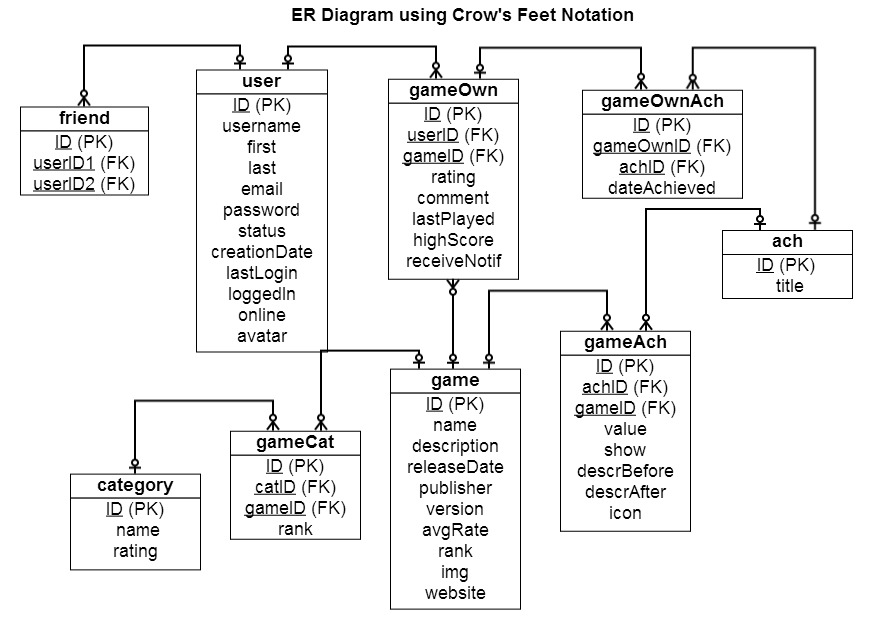
\includegraphics[width=0.75\columnwidth]{er} % Import image
\end{center}

\chapter{\textbf{Appendix B: Data Types}}
\begin{center}
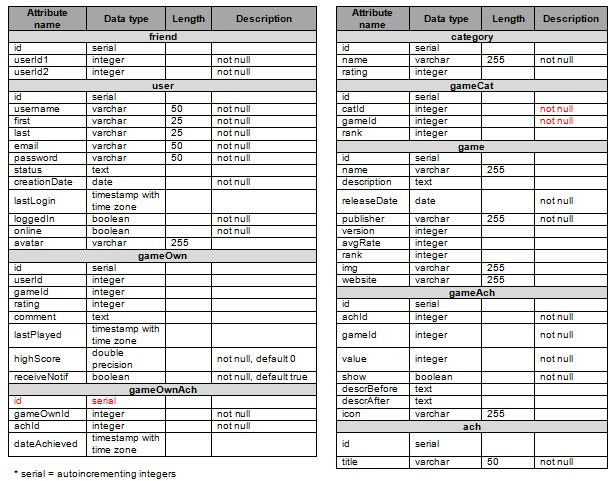
\includegraphics[width=0.67\columnwidth]{types} % Import image
\end{center}

\chapter{\textbf{Appendix C: Mark Allocation}}
\begin{center}
    \begin{tabular}{| l | c | c |}
    \hline
    \textbf{Name} & \textbf{Allocated Mark} & \textbf{Signature} \\ \hline
    Liban Abdulkadir & 0.25 & L.A \\ \hline
    Ana Dumitra\c{s} & 0.25 & A.D \\ \hline
    Andra Irimia & 0.25 & A.I \\ \hline
    Ioan Troan\v{a} & 0.25 & I.T \\ \hline
    \end{tabular}
\end{center}

% To have just one problem per page, simply put a \clearpage after each problem

%\begin{homeworkProblem}
%Listing \ref{homework_example} shows a Perl script.

%\perlscript{homework_example}{Sample Perl Script With Highlighting}

%\end{homeworkProblem}

%----------------------------------------------------------------------------------------
%	PROBLEM 2
%----------------------------------------------------------------------------------------

%\begin{homeworkProblem}

%\problemAnswer{
%\begin{center}
%\includegraphics[width=0.75\columnwidth]{example_figure} % Example image
%\end{center}

%}
%\end{homeworkProblem}

%----------------------------------------------------------------------------------------

\end{document}
